% ============================================================
%  Section 3 — Methodology
%  Describes the proposed framework in generic terms (notation,
%  equations, design rationale). Dataset-specific values (window
%  length, thresholds, partition sizes) and hyperparameters are
%  given in Section 4; all measured outcomes are in Section 5.
%
%  Packages needed (preamble): amsmath, amssymb, algorithm,
%  algpseudocode, graphicx, booktabs.
%
%  Figure needed: figures/framework_overview.png (Lucid export)
% ============================================================

\section{Methodology}
\label{sec:methodology}

This section presents the proposed framework. Its overall structure
is given first, followed by the notation, the automatic construction
of degradation stages and RUL targets, and the three contributions:
stage-conditioned generative augmentation, multi-task prediction, and
stage-conditional cross-conformal calibration.

% ------------------------------------------------------------
\subsection{Framework Overview}
\label{sec:method_overview}

Fig.~\ref{fig:framework} summarises the framework. Raw vibration
recordings are first converted into multivariate feature vectors and
a scalar health indicator. The health indicator is used to place two
landmarks on each bearing's trajectory, the First Prediction Time and
an acceleration point, which define three degradation stages and a
piecewise RUL target without manual annotation. The feature vectors
are then segmented into fixed-length windows. The test bearings are
set aside, and the remaining bearings are used in turn for training
and for calibration through a cross-conformal scheme, so that every
non-test bearing contributes to calibration without ever being scored
by a model trained on it.\\

The three contributions act at successive points of this pipeline.
The stage-conditioned generator (C1) is trained on the training
partition and produces synthetic near-failure windows, which enter
the training set only. The multi-task predictor (C2) is trained on
this augmented set to estimate the RUL and the degradation stage
jointly from a shared representation. Finally, the stage-conditional
cross-conformal procedure (C3) uses the out-of-sample errors of the
predictor on real bearings to turn each point prediction into an
interval, and conditions that interval on the stage predicted by the
stage head of C2.\\

One constraint governs the whole pipeline: synthetic data never
reaches the calibration or test partitions. The coverage guarantee of
conformal prediction rests on the calibration and test samples being
exchangeable. Synthetic windows follow the distribution learned by the
generator, not the true data distribution, so admitting them into
calibration would measure the predictor's error against the wrong
reference. Augmentation is therefore confined to training, where it
can only change the predictor, and the guarantee is preserved.

\begin{figure*}[!htbp]
  \centering
  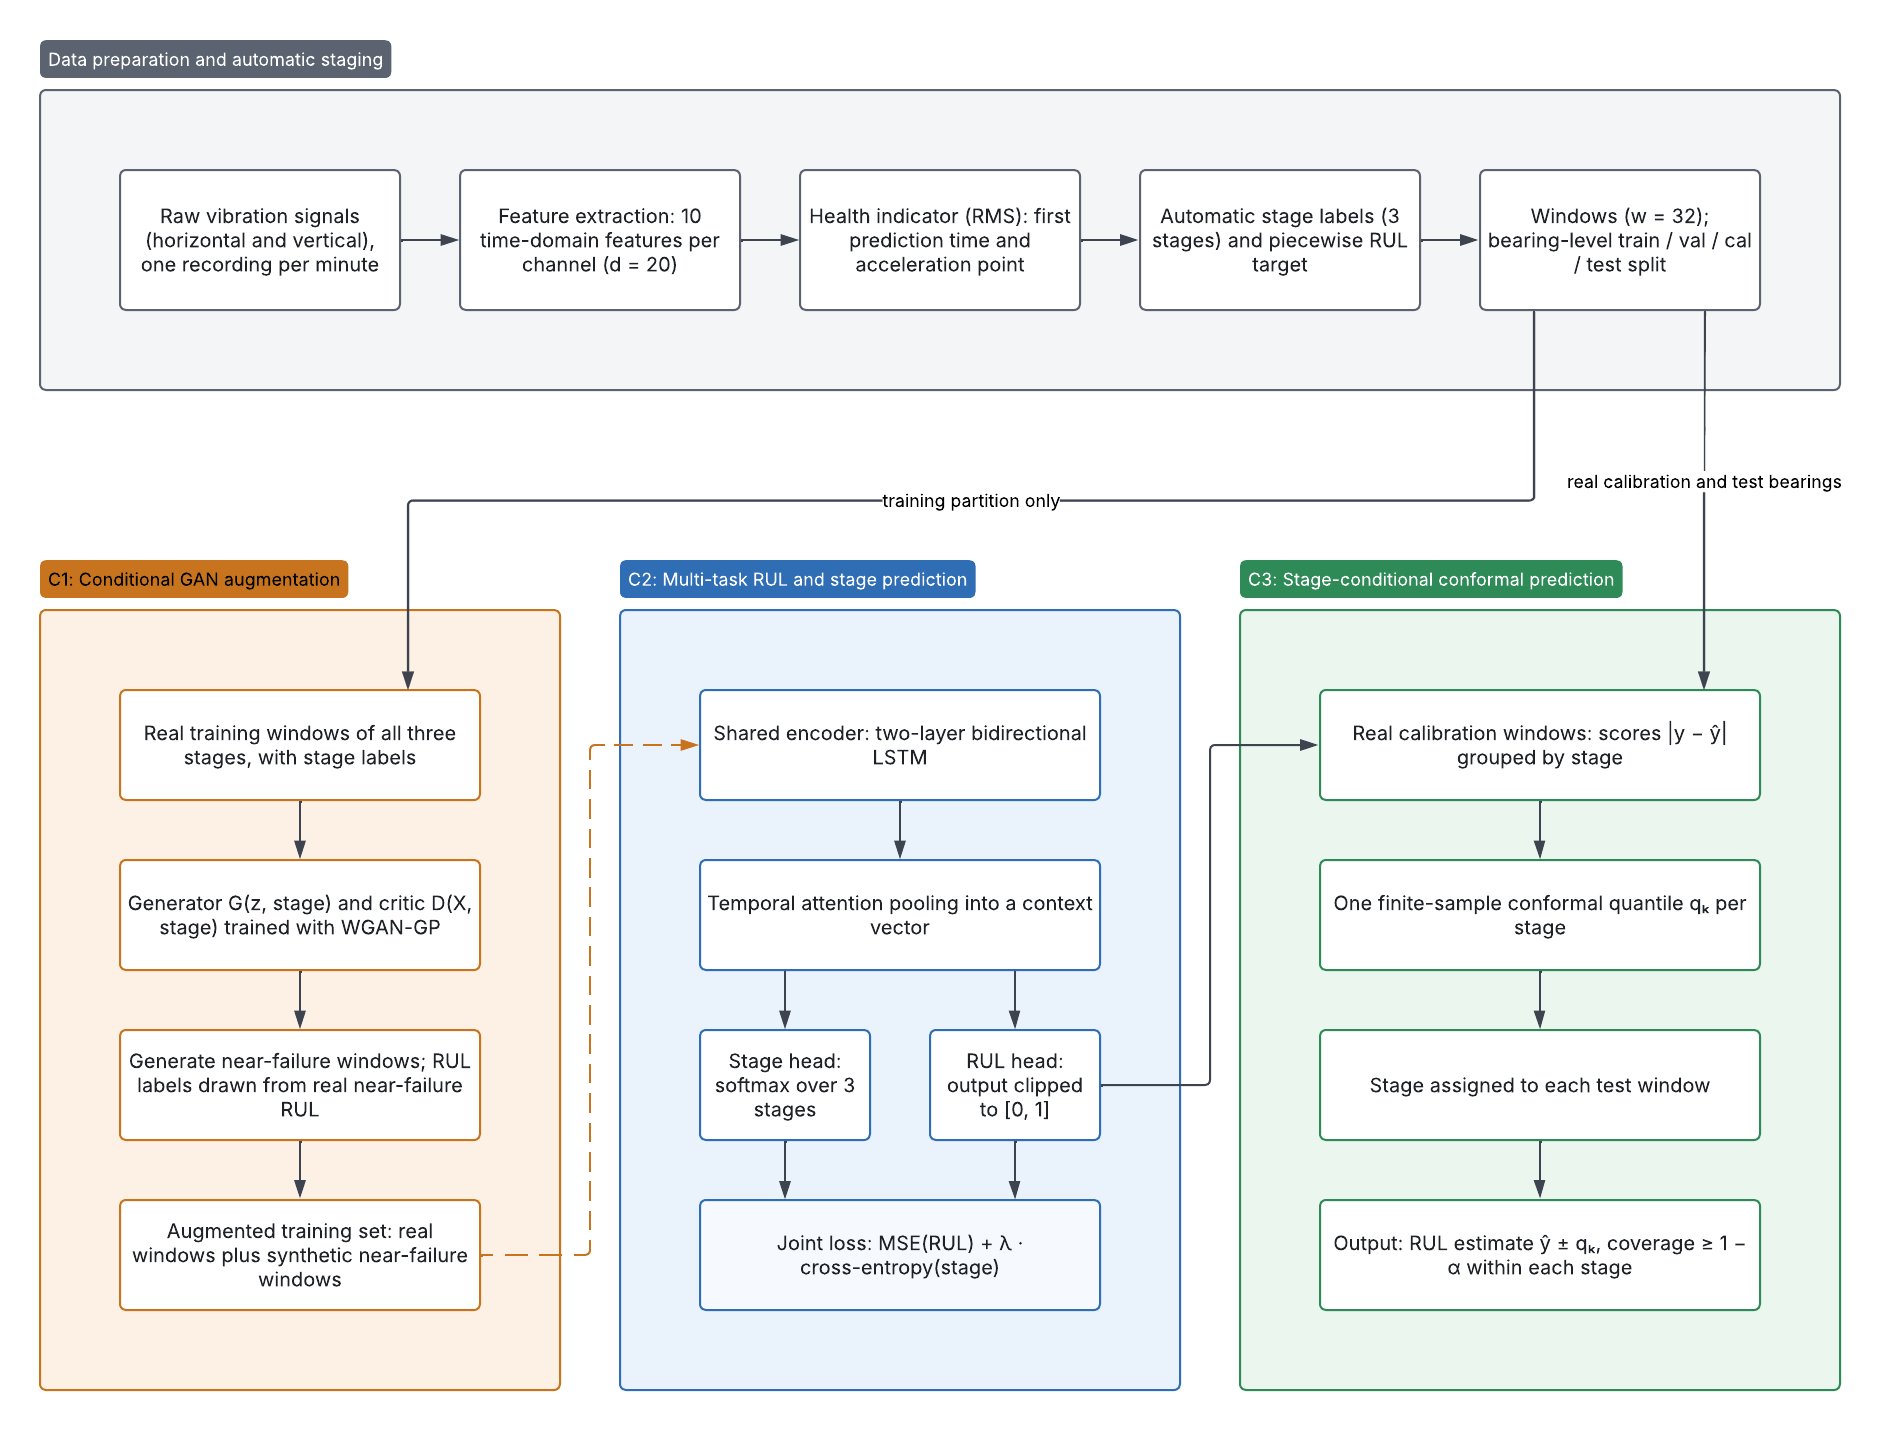
\includegraphics[width=\textwidth]{figures/framework_overview.png}
  \caption{Overview of the proposed framework. Synthetic windows
  produced by the stage-conditioned generator (C1) enter the training
  set only (dashed arrow); calibration and test use real recordings
  exclusively. The RUL head of the multi-task predictor (C2) supplies the
  point estimates whose out-of-sample residuals define the conformal
  intervals, and its stage head supplies the stage on which the interval
  is conditioned (C3).}
  \label{fig:framework}
\end{figure*}

% ------------------------------------------------------------
\subsection{Problem Formulation}
\label{sec:method_notation}

Consider a set of bearings $\mathcal{B}$, each monitored from its
first recording to failure. For bearing $b \in \mathcal{B}$ with
lifetime $T_b$ recordings, a feature vector
$\mathbf{x}^{b}_{t} \in \mathbb{R}^{d}$ is extracted from the
recording at time $t = 1, \dots, T_b$. The model input at time $t$ is
the window of the $w$ most recent feature vectors,
\begin{equation}
  \mathbf{X}^{b}_{t} =
  \left[\mathbf{x}^{b}_{t-w+1}, \dots, \mathbf{x}^{b}_{t}\right]
  \in \mathbb{R}^{w \times d}, \qquad t \geq w,
  \label{eq:window}
\end{equation}
which contains no information posterior to $t$. Each window carries
two labels taken at its final time step: a normalised RUL target
$y^{b}_{t} \in [0,1]$ and a degradation stage
$s^{b}_{t} \in \{1, 2, 3\}$, both defined in
Section~\ref{sec:method_staging}.\\

For a given model, the bearings are split into disjoint training,
validation, calibration and test sets, denoted
$\mathcal{D}_{\mathrm{tr}}$, $\mathcal{D}_{\mathrm{val}}$,
$\mathcal{D}_{\mathrm{cal}}$ and $\mathcal{D}_{\mathrm{te}}$, at the
level of whole bearings. This choice follows from
Eq.~\eqref{eq:window}: consecutive windows of the same bearing share
$w-1$ of their $w$ time steps, so a window-level split would place
near-duplicates on both sides of the training--calibration boundary.
Section~\ref{sec:c3_conformal} describes how these roles rotate among
the non-test bearings.\\

The objective is twofold. The first is a point predictor
$\hat{f}: \mathbb{R}^{w \times d} \to [0,1]$ with small error on
unseen bearings, particularly in the near-failure stage. The second is
an interval predictor $\hat{C}(\mathbf{X})$ that satisfies, for a
user-chosen miscoverage level $\alpha$, the stage-conditional coverage
property
\begin{equation}
  \mathbb{P}\left( y \in \hat{C}(\mathbf{X}) \;\middle|\; s = k \right)
  \geq 1 - \alpha, \qquad k \in \{1, 2, 3\}.
  \label{eq:coverage_goal}
\end{equation}
Coverage within each stage is required, rather than coverage averaged
over all windows, because the stages differ sharply in size and
difficulty. An average dominated by the abundant healthy windows can
satisfy the nominal level while the near-failure stage, the one that
drives maintenance decisions, is under-covered.

% ------------------------------------------------------------
\subsection{Automatic Degradation Staging and RUL Target}
\label{sec:method_staging}

Stage labels and RUL targets are derived from a scalar health
indicator (HI) rather than annotated by hand. The HI $h_t$ is the root
mean square of one vibration channel, computed per recording and
smoothed with a short moving average.\\

The First Prediction Time $t_{\mathrm{F}}$ marks the end of the healthy
regime. A healthy baseline with mean $\mu_b$ and standard deviation
$\sigma_b$ is estimated from the initial fraction $\eta$ of the
bearing's life. The detection threshold is the stricter of a
statistical criterion and a relative floor,
\begin{equation}
  \tau_b = \max\left( \mu_b + 3\sigma_b,\; (1+\rho)\,\mu_b \right),
  \label{eq:fpt_threshold}
\end{equation}
and the FPT is the first instant from which the HI stays above
$\tau_b$ for $m$ consecutive recordings,
\begin{equation}
  t_{\mathrm{F}} = \min \left\{ t \;:\; h_{t+j} > \tau_b,
  \;\; j = 0, \dots, m-1 \right\}.
  \label{eq:fpt}
\end{equation}
The two terms of Eq.~\eqref{eq:fpt_threshold} play distinct roles. The
statistical term rejects departures that are small compared with the
baseline noise. The relative term $\rho$ guards against bearings whose
baseline is so stable that $\sigma_b$ is close to zero, in which case
$\mu_b + 3\sigma_b$ alone would be crossed by ordinary fluctuations.
The persistence length $m$ in Eq.~\eqref{eq:fpt} prevents a single
transient from being taken as a change of regime.\\

Within the degradation phase, an acceleration point $t_{\mathrm{A}}$
separates gradual from severe degradation. Let
$\Delta h_t = h_t - h_{t-1}$ denote the first difference of the HI.
Its mean $\mu_\Delta$ and standard deviation $\sigma_\Delta$ are
estimated over the first half of the interval
$[t_{\mathrm{F}}, T_b]$, and $t_{\mathrm{A}}$ is the first instant in
the second half at which
\begin{equation}
  \Delta h_t > \mu_\Delta + \sigma_\Delta .
  \label{eq:acc_point}
\end{equation}
When no such instant exists, $t_{\mathrm{A}}$ is placed at 70\% of the
degradation interval. The two landmarks define the stage of every
recording,
\begin{equation}
  s_t =
  \begin{cases}
    1 & t < t_{\mathrm{F}} \quad \text{(healthy)},\\
    2 & t_{\mathrm{F}} \leq t < t_{\mathrm{A}}
        \quad \text{(early degradation)},\\
    3 & t \geq t_{\mathrm{A}} \quad \text{(near-failure)}.
  \end{cases}
  \label{eq:stages}
\end{equation}

The RUL target is defined piecewise from the same landmark:
\begin{equation}
  y_t =
  \begin{cases}
    1 & t < t_{\mathrm{F}},\\[2pt]
    \dfrac{T_b - t}{T_b - t_{\mathrm{F}}} & t \geq t_{\mathrm{F}}.
  \end{cases}
  \label{eq:rul_target}
\end{equation}
The target is held at unity during the healthy phase and decreases
linearly to zero at failure. A target that decreases from the first
recording would give different labels to healthy windows whose
signals are nearly identical, a mapping the predictor cannot learn.
Because healthy windows are the most numerous, such a target also
biases the predictor toward overestimating the remaining life, which
is the unsafe direction of error. Normalising by the length of the
degradation phase keeps the target on a common scale across bearings
whose lifetimes may differ by orders of magnitude.

% ------------------------------------------------------------
\subsection{Stage-Conditioned Generative Augmentation (C1)}
\label{sec:c1_gan}

The near-failure stage is the least represented in run-to-failure data
and the most important for maintenance. C1 enlarges it with synthetic
windows produced by a conditional generative adversarial network. The
generator produces complete multivariate windows of dimension
$w \times d$, rather than a scalar degradation curve, so that the
correlations between features and between channels are reproduced.\\

\textit{Architecture.} The generator $G$ receives a noise vector
$\mathbf{z} \sim \mathcal{N}(\mathbf{0}, \mathbf{I})$ concatenated with
a one-hot encoding $\mathbf{e}_c$ of the requested stage $c$. A linear
layer projects this input into a short seed sequence, two
one-dimensional convolutional layers extract local patterns, and a
bidirectional LSTM models the temporal dependencies before a linear
layer outputs the window $\tilde{\mathbf{X}} = G(\mathbf{z},
\mathbf{e}_c)$. The critic $D$ receives a window together with the same
stage encoding, repeated at every time step, and passes it through two
convolutional layers and a bidirectional LSTM. The final hidden state
is layer-normalised and mapped to an unbounded scalar score. Layer
normalisation is used instead of batch normalisation because the
gradient penalty below is defined per sample.\\

Conditioning both networks on the stage is what allows a specific
regime to be requested. An unconditional generator would reproduce the
distribution of its training data, which is dominated by healthy
windows, and leave the scarcity unaddressed. The generator is
therefore trained on windows of all three stages, so that it learns
how the stages differ, and is queried only for $c = 3$ at
augmentation time.\\

\textit{Training objective.} Training follows the Wasserstein
formulation with gradient penalty~\cite{NIPS2017_892c3b1c}, chosen for
its resistance to mode collapse. A collapsed generator would emit
near-identical windows and add no information to the training set.
The critic minimises
\begin{equation}
  \mathcal{L}_{D} =
  \mathbb{E}\big[ D(\tilde{\mathbf{X}}, \mathbf{e}_c) \big]
  - \mathbb{E}\big[ D(\mathbf{X}, \mathbf{e}_c) \big]
  + \lambda_{\mathrm{gp}}\,
  \mathbb{E}\Big[ \big( \lVert \nabla_{\hat{\mathbf{X}}}
  D(\hat{\mathbf{X}}, \mathbf{e}_c) \rVert_2 - 1 \big)^2 \Big],
  \label{eq:critic_loss}
\end{equation}
where $\mathbf{X}$ is a real window of stage $c$, $\tilde{\mathbf{X}}$
a generated window of the same stage, and
$\hat{\mathbf{X}} = \epsilon \mathbf{X} + (1-\epsilon)
\tilde{\mathbf{X}}$ with $\epsilon \sim \mathcal{U}(0,1)$. The last
term enforces the Lipschitz constraint on which the Wasserstein
estimate depends. The generator minimises
\begin{equation}
  \mathcal{L}_{G} =
  - \mathbb{E}\big[ D(G(\mathbf{z}, \mathbf{e}_c), \mathbf{e}_c) \big],
  \label{eq:gen_loss}
\end{equation}
and is updated once for every $n_{\mathrm{c}}$ critic updates. A
separate generator is trained for every predictor, on that predictor's
training windows only, so that no synthetic window derives from a
bearing later used to calibrate it.\\

\textit{Augmentation and labelling.} Let $N_3$ be the number of real
near-failure windows in $\mathcal{D}_{\mathrm{tr}}$. For an
augmentation ratio $r$, the generator produces
$\lfloor r N_3 \rceil$ windows with $c = 3$, and these are added to the
training set with stage label 3. Each synthetic window also needs an
RUL label, which the generator does not provide because it is
conditioned on the stage and not on the RUL. The label is drawn at
random, with replacement, from the empirical distribution of the RUL
values of the real near-failure training windows,
\begin{equation}
  \tilde{y} \sim \mathrm{Unif}\left\{ y_i \;:\; s_i = 3,\;
  i \in \mathcal{D}_{\mathrm{tr}} \right\}.
  \label{eq:syn_label}
\end{equation}
This preserves the marginal distribution of near-failure RUL values in
the augmented set, so the augmentation does not shift the predictor
toward any particular value. The augmented set
$\mathcal{D}_{\mathrm{tr}}^{+} = \mathcal{D}_{\mathrm{tr}} \cup
\mathcal{D}_{\mathrm{syn}}$ replaces $\mathcal{D}_{\mathrm{tr}}$ for
training the predictor. The validation, calibration and test sets are
left unchanged.

% ------------------------------------------------------------
\subsection{Multi-task RUL and Stage Prediction (C2)}
\label{sec:c2_multitask}

The predictor estimates the RUL and the degradation stage jointly from
a shared encoder. The auxiliary stage task asks the encoder to
separate the three regimes, which are the same regimes in which the
RUL behaves differently. The stage labels come from
Eq.~\eqref{eq:stages} and therefore cost no annotation.\\

\textit{Shared encoder.} A two-layer bidirectional LSTM maps the input
window to a sequence of hidden states
$\mathbf{H} = [\mathbf{h}_1, \dots, \mathbf{h}_w]$, where each
$\mathbf{h}_k$ concatenates the forward and backward states. A temporal
attention layer pools this sequence into a context vector,
\begin{equation}
  a_k = \mathbf{v}^{\top} \tanh\left( \mathbf{W}_a \mathbf{h}_k +
  \mathbf{b}_a \right), \qquad
  \beta_k = \frac{\exp(a_k)}{\sum_{j=1}^{w} \exp(a_j)}, \qquad
  \mathbf{c} = \sum_{k=1}^{w} \beta_k \mathbf{h}_k ,
  \label{eq:attention}
\end{equation}
so that the time steps most informative about the current state of
degradation receive the largest weights.\\

\textit{Task heads.} Two heads read the context vector $\mathbf{c}$.
The RUL head is a small feed-forward network whose output is clipped to
the unit interval,
\begin{equation}
  \hat{y} = \min\left( 1, \max\left( 0, \; g_{\mathrm{rul}}(\mathbf{c})
  \right) \right).
  \label{eq:rul_head}
\end{equation}
Clipping is preferred to a sigmoid output because the target of
Eq.~\eqref{eq:rul_target} takes the exact value 1 on every healthy
window, a value a sigmoid only approaches asymptotically. The stage
head is a feed-forward network followed by a softmax over the three
stages, giving the predicted probabilities
$\hat{\mathbf{p}} = \mathrm{softmax}(g_{\mathrm{st}}(\mathbf{c}))$.\\

\textit{Joint objective.} Both heads are trained together on every
window of $\mathcal{D}_{\mathrm{tr}}^{+}$ by minimising
\begin{equation}
  \mathcal{L} = \frac{1}{N} \sum_{i=1}^{N} \left( \hat{y}_i - y_i
  \right)^2
  \;-\; \lambda \, \frac{1}{N} \sum_{i=1}^{N} \log \hat{p}_{i,\,s_i},
  \label{eq:mt_loss}
\end{equation}
where $\lambda \geq 0$ weights the stage loss. Setting $\lambda = 0$
and removing the stage head recovers the single-task predictor used as
the baseline. Healthy windows enter both terms: the piecewise target
makes their RUL learnable, and in the stage term they supply the
examples the encoder needs to recognise the healthy regime. Training
stops when the RUL error on $\mathcal{D}_{\mathrm{val}}$ has not
improved for a fixed number of epochs, and the weights with the lowest
validation error are retained.


% ------------------------------------------------------------
\subsection{Stage-Conditional Cross-Conformal Prediction (C3)}
\label{sec:c3_conformal}

C3 converts the point prediction into an interval with a
distribution-free coverage guarantee. It makes no assumption about the
predictor or the error distribution, and it is applied after training,
so it leaves the predictor unchanged~\cite{lei2018distribution,
angelopoulos2023gentle}.\\

\textit{Split conformal prediction.} In its simplest form, a trained
predictor $\hat{f}$ is applied to a held-out calibration set, and each
calibration window receives the nonconformity score
\begin{equation}
  r_i = \left| y_i - \hat{f}(\mathbf{X}_i) \right|,
  \qquad i \in \mathcal{D}_{\mathrm{cal}} .
  \label{eq:score}
\end{equation}
With the $n$ scores sorted in increasing order,
$r_{(1)} \leq \dots \leq r_{(n)}$, the interval for a new window is
$\hat{f}(\mathbf{X}) \pm \hat{q}$ with
\begin{equation}
  \hat{q} = r_{(k)}, \qquad
  k = \left\lceil (n+1)(1-\alpha) \right\rceil .
  \label{eq:quantile}
\end{equation}
The correction $(n+1)$ yields the finite-sample guarantee
$\mathbb{P}(y \in \hat{C}(\mathbf{X})) \geq 1 - \alpha$ whenever the
calibration and test windows are exchangeable.\\

\textit{Why a single calibration split is insufficient.} Exchangeability
must hold between bearings, not only between windows, because the
windows of one bearing are strongly dependent. A run-to-failure dataset
contains few bearings, and every bearing assigned to calibration is
removed from training. A held-out calibration set therefore represents
the variability between bearings through very few units, and the
intervals inherit whatever is specific to those units. The framework
avoids this by using every non-test bearing for calibration through
cross-conformal prediction.\\

\textit{Cross-conformal calibration (CV+).} The non-test bearings are
divided into $K$ disjoint groups $\mathcal{G}_1, \dots, \mathcal{G}_K$.
For each $j$, a predictor $\hat{f}_{-j}$ is trained without the
bearings of $\mathcal{G}_j$, including its own generator (C1), feature
scaler and early stopping, and is applied to the windows of
$\mathcal{G}_j$. Every non-test window $i$ thus receives an
out-of-sample score
\begin{equation}
  R_i = \left| y_i - \hat{f}_{-j(i)}(\mathbf{X}_i) \right|,
  \label{eq:oof_score}
\end{equation}
where $j(i)$ is the group containing the bearing of window $i$. For a
test window $\mathbf{X}$, each score is combined with the prediction of
the model that produced it, and the CV+
interval~\cite{barber2021jackknife} is
\begin{equation}
  \hat{C}(\mathbf{X}) = \Big[\,
  \hat{q}^{-}_{\alpha}\big\{ \hat{f}_{-j(i)}(\mathbf{X}) - R_i \big\},\;
  \hat{q}^{+}_{\alpha}\big\{ \hat{f}_{-j(i)}(\mathbf{X}) + R_i \big\}
  \,\Big],
  \label{eq:cvplus}
\end{equation}
where, over the $n$ values in braces, $\hat{q}^{+}_{\alpha}$ is the
$\lceil (1-\alpha)(n+1) \rceil$-th smallest value and
$\hat{q}^{-}_{\alpha}$ the $\lfloor \alpha (n+1) \rfloor$-th smallest.
If the $K$ models gave identical predictions, Eq.~\eqref{eq:cvplus}
would reduce to the split interval of Eq.~\eqref{eq:quantile}; it
accounts for their disagreement otherwise. The guarantee is
$1 - 2\alpha$ in the worst case and close to $1 - \alpha$ in
practice~\cite{barber2021jackknife}. The point estimate is the mean of
the $K$ predictions, $\bar{f}(\mathbf{X}) = K^{-1}\sum_j
\hat{f}_{-j}(\mathbf{X})$. Because the RUL lies in $[0,1]$, the
interval is finally intersected with the unit interval, which removes
impossible values without changing coverage.\\

\textit{Conditioning on the predicted stage.} The coverage of
Eq.~\eqref{eq:cvplus} holds on average over all windows, which is
weaker than the requirement of Eq.~\eqref{eq:coverage_goal}. When the
scores of different stages follow different distributions, a single
interval width is too wide for some stages and too narrow for others.
Following the Mondrian construction~\cite{vovk2005algorithmic}, the
calibration windows are partitioned into groups and the quantiles of
Eq.~\eqref{eq:cvplus} are taken within the group of the test window
only. The group must be computable for a bearing in service. The
landmarks of Section~\ref{sec:method_staging} are located from the
complete trajectory, so the true stage is not available before failure.
The group is therefore the stage predicted from the window,
$\hat{s} = \arg\max_k \hat{p}_k$. Each calibration window takes the
stage predicted by the stage head of the model that did not see it,
and a test window takes the stage that maximises the average of the
$K$ stage heads' probabilities. Because $\hat{s}$ depends on the input
only, the guarantee holds within each predicted stage; coverage within
the true stages is measured empirically in Section~\ref{sec:results}.\\

In the multi-task configurations this links C2 and C3 directly: the
stage head that shapes the shared representation during training also
supplies the stage on which the interval is conditioned, so a single
network provides the RUL estimate, the stage and the interval. In the
single-task configurations, which have no stage head, the stage is
provided by a separate network with the same encoder and stage head,
trained on the same real training windows.\\

Three design choices protect the exchangeability on which these
guarantees rest. Partitioning is done at the bearing level, so that no
calibration window has a near-duplicate in the training data of the
model that scores it. Synthetic windows are confined to training, and
each generator is trained only on the bearings of its own predictor,
so that calibration measures the error against real, unseen data.
Finally, every non-test bearing contributes to calibration, so that
the calibration population reflects the variability between bearings
as fully as the dataset allows.

% ------------------------------------------------------------
\subsection{Training and Evaluation Procedure}
\label{sec:method_procedure}

Algorithm~\ref{alg:framework} summarises the procedure for one set of
test bearings. The four configurations compared in
Section~\ref{sec:results} are obtained by switching C1 and C2 on or
off: the baseline uses neither ($r = 0$, $\lambda = 0$), the augmented
configuration uses C1 only, the multi-task configuration uses C2 only,
and the full framework uses both. C3 is applied identically to all
four, so that differences in the intervals can be attributed to the
predictor.

\begin{algorithm}[!htbp]
\caption{Proposed framework for one set of test bearings.}
\label{alg:framework}
\begin{algorithmic}[1]
\Require Test bearings $\mathcal{D}_{\mathrm{te}}$; non-test bearings
         in groups $\mathcal{G}_1, \dots, \mathcal{G}_K$; ratio $r$;
         weight $\lambda$; level $\alpha$
\State Compute $t_{\mathrm{F}}$, $t_{\mathrm{A}}$, $s_t$ and $y_t$ for
       every bearing \Comment{Eqs.~\eqref{eq:fpt}--\eqref{eq:rul_target}}
\For{$j = 1, \dots, K$}
  \State $\mathcal{D}_{\mathrm{tr}}, \mathcal{D}_{\mathrm{val}} \gets$
         non-test bearings outside $\mathcal{G}_j$
  \State Fit the feature scaler on $\mathcal{D}_{\mathrm{tr}}$
  \If{$r > 0$} \Comment{C1}
    \State Train $(G, D)$ on $\mathcal{D}_{\mathrm{tr}}$; generate
           $\lfloor r N_3 \rceil$ windows with $c=3$, labelled by
           Eq.~\eqref{eq:syn_label}
  \EndIf
  \State Train $\hat{f}_{-j}$ on $\mathcal{D}_{\mathrm{tr}}^{+}$ with
         Eq.~\eqref{eq:mt_loss}; early-stop on $\mathcal{D}_{\mathrm{val}}$
         \Comment{C2}
  \State Score $\mathcal{G}_j$: $R_i$ by Eq.~\eqref{eq:oof_score} and
         $\hat{s}_i$ from the stage head
  \State Predict $\mathcal{D}_{\mathrm{te}}$: RUL and stage probabilities
\EndFor
\For{each $\mathbf{X} \in \mathcal{D}_{\mathrm{te}}$} \Comment{C3}
  \State $\hat{s} \gets$ stage of the averaged probabilities;
         $\bar{f}(\mathbf{X}) \gets$ mean of the $K$ predictions
  \State $\hat{C}(\mathbf{X}) \gets$ Eq.~\eqref{eq:cvplus} over the
         calibration windows with $\hat{s}_i = \hat{s}$, clipped to $[0,1]$
\EndFor
\end{algorithmic}
\end{algorithm}
